% The methods used in this study are briefly described and listed in order of execution in \tref{tbl:methods}. Furthermore, detailed explanations of key concepts are presented throughout the rest of the section. 
GIS-based methods were selected to model the current state of the basin and evaluate treated wastewater reuse scenarios. By incorporating the spatial distribution of resources in WEF Nexus modelling and preventing aggregation of spatial scales, more robust analytical analysis tackling the intersection of all three resources can be achieved, providing better insights for planning and decision making \cite{shannakMovingTheoryPractice2018,albrechtWaterEnergyFoodNexusSystematic2018}. This concept gains even more importance in the context of the transboundary nature of the NWSAS basin.

The most up-to-date open source data available was collected and processed. The relevant layers are identified and described in \textit{section 1} of the \textit{supplementary information}. A general model and case study runner for the NWSAS were developed using Python and hosted in an open-source \href{https://github.com/camiloramirezgo/NWSAS-paper-model}{\textbf{Github repository}} which ensures the complete reproducibility of the results.

Throughout this section, the methods used to characterise the current state of the aquifer (Baseline scenario) are presented. Then, descriptions of the treated wastewater reuse scenarios are provided along with the methods used and a schematic representation of the overall system. Finally, detailed explanations of key modelling processes are given.

\subsection{Characterizing the Baseline scenario}
Water requirements for domestic and irrigation use were assumed to be supplied by the groundwater aquifer, whereas other water uses were excluded as they are considered insignificant. The recharge rate $R$ for the entire aquifer was taken as 1.1 billion cubic meters of water per year, which for the area of the aquifer, is an equivalent water column of 1.06 mm per year \cite{BetterValorizationIrrigation2015}. Furthermore, no environmental flow, wastewater treatment or reuse were considered.

\begin{table*}[!b]
    \caption{\label{tbl:methodsBaseline}Brief description and enumeration of methods used for the Baseline scenario (in order of execution).}
	\footnotesize
	\begin{tabular*}{\textwidth}{@{}l P{1.1in} P{1.2in} P{3.12in}}
		\br
		\# & Method & Systems involved & Description\\
		\mr
	    1. & Data calibration & Residential and agriculture & Geospatial population count and irrigated cropland extend calibrated according to provincial statistics\\
	    2. & Clustering & Residential and agricultural sectors & Clusters of population and cropland extent points are identified\\
	    3. & Water demand & Residential and agriculture & Based on population water consumption per capita and spatial irrigation water needs per hectare according to provincial statistics \\
	    4. & Water withdrawals & Groundwater aquifer, residential and agriculture & Calculate water withdrawals from the groundwater aquifer, based on demand from the residential and agricultural sectors. No water reuse is accounted here\\
	    5. & Groundwater stress indicator & Groundwater aquifer & Estimate geospatially the current groundwater stress indicator based on the water extractions, the recharge rate of the aquifer and the areal extent of each cluster and the basin\\
	    6. & Pumping energy & Groundwater aquifer & Based on total water withdrawals from the aquifer and the depth to groundwater of each spatial location \\
		\br
	\end{tabular*}
\end{table*}

Water demand for domestic use was estimated using a low level water demand per capita of 55 m\textsuperscript{3}/year \cite{Householdwaterconsumption2014}, based on medium consumption values recommended by the World Health Organization to prevent health risks. Current population was set according to statistics from population count withing each country area inside the basin \cite{BetterValorizationIrrigation2015}, with an annual growth of 2\% for the Algerian and Libyan parts and 1\% for the Tunisian part \cite{uneceReconcilingResourceUses2020}. The agricultural irrigation requirements were taken from provincial specific data derived from \cite{Socioeconomicaspectsirrigation2014}. Moreover, irrigated area was also taken from provincial data from \cite{Socioeconomicaspectsirrigation2014,BetterValorizationIrrigation2015,almullaNWSAS} and irrigated area growth was considered based on irrigation intensification rates (i.e. describe the current average rate of irrigated area over the feasible area to be irrigated in each region) \cite{Socioeconomicaspectsirrigation2014}. Details of such data is provided in the \textit{supplementary information}.

Finally, the analysis was done for an average year between a period of 35 years spanning from year 2015 to 2050. This time period was selected to account for the lifespan of the treatment technologies evaluated in the treated wastewater/tailwater scenarios.

\Tref{tbl:methodsBaseline} presents the six main steps performed in order to characterize the current state of the basin.

\subsection{Wastewater treatment and reuse scenarios}
\begin{figure*}[!b]
	\centering
	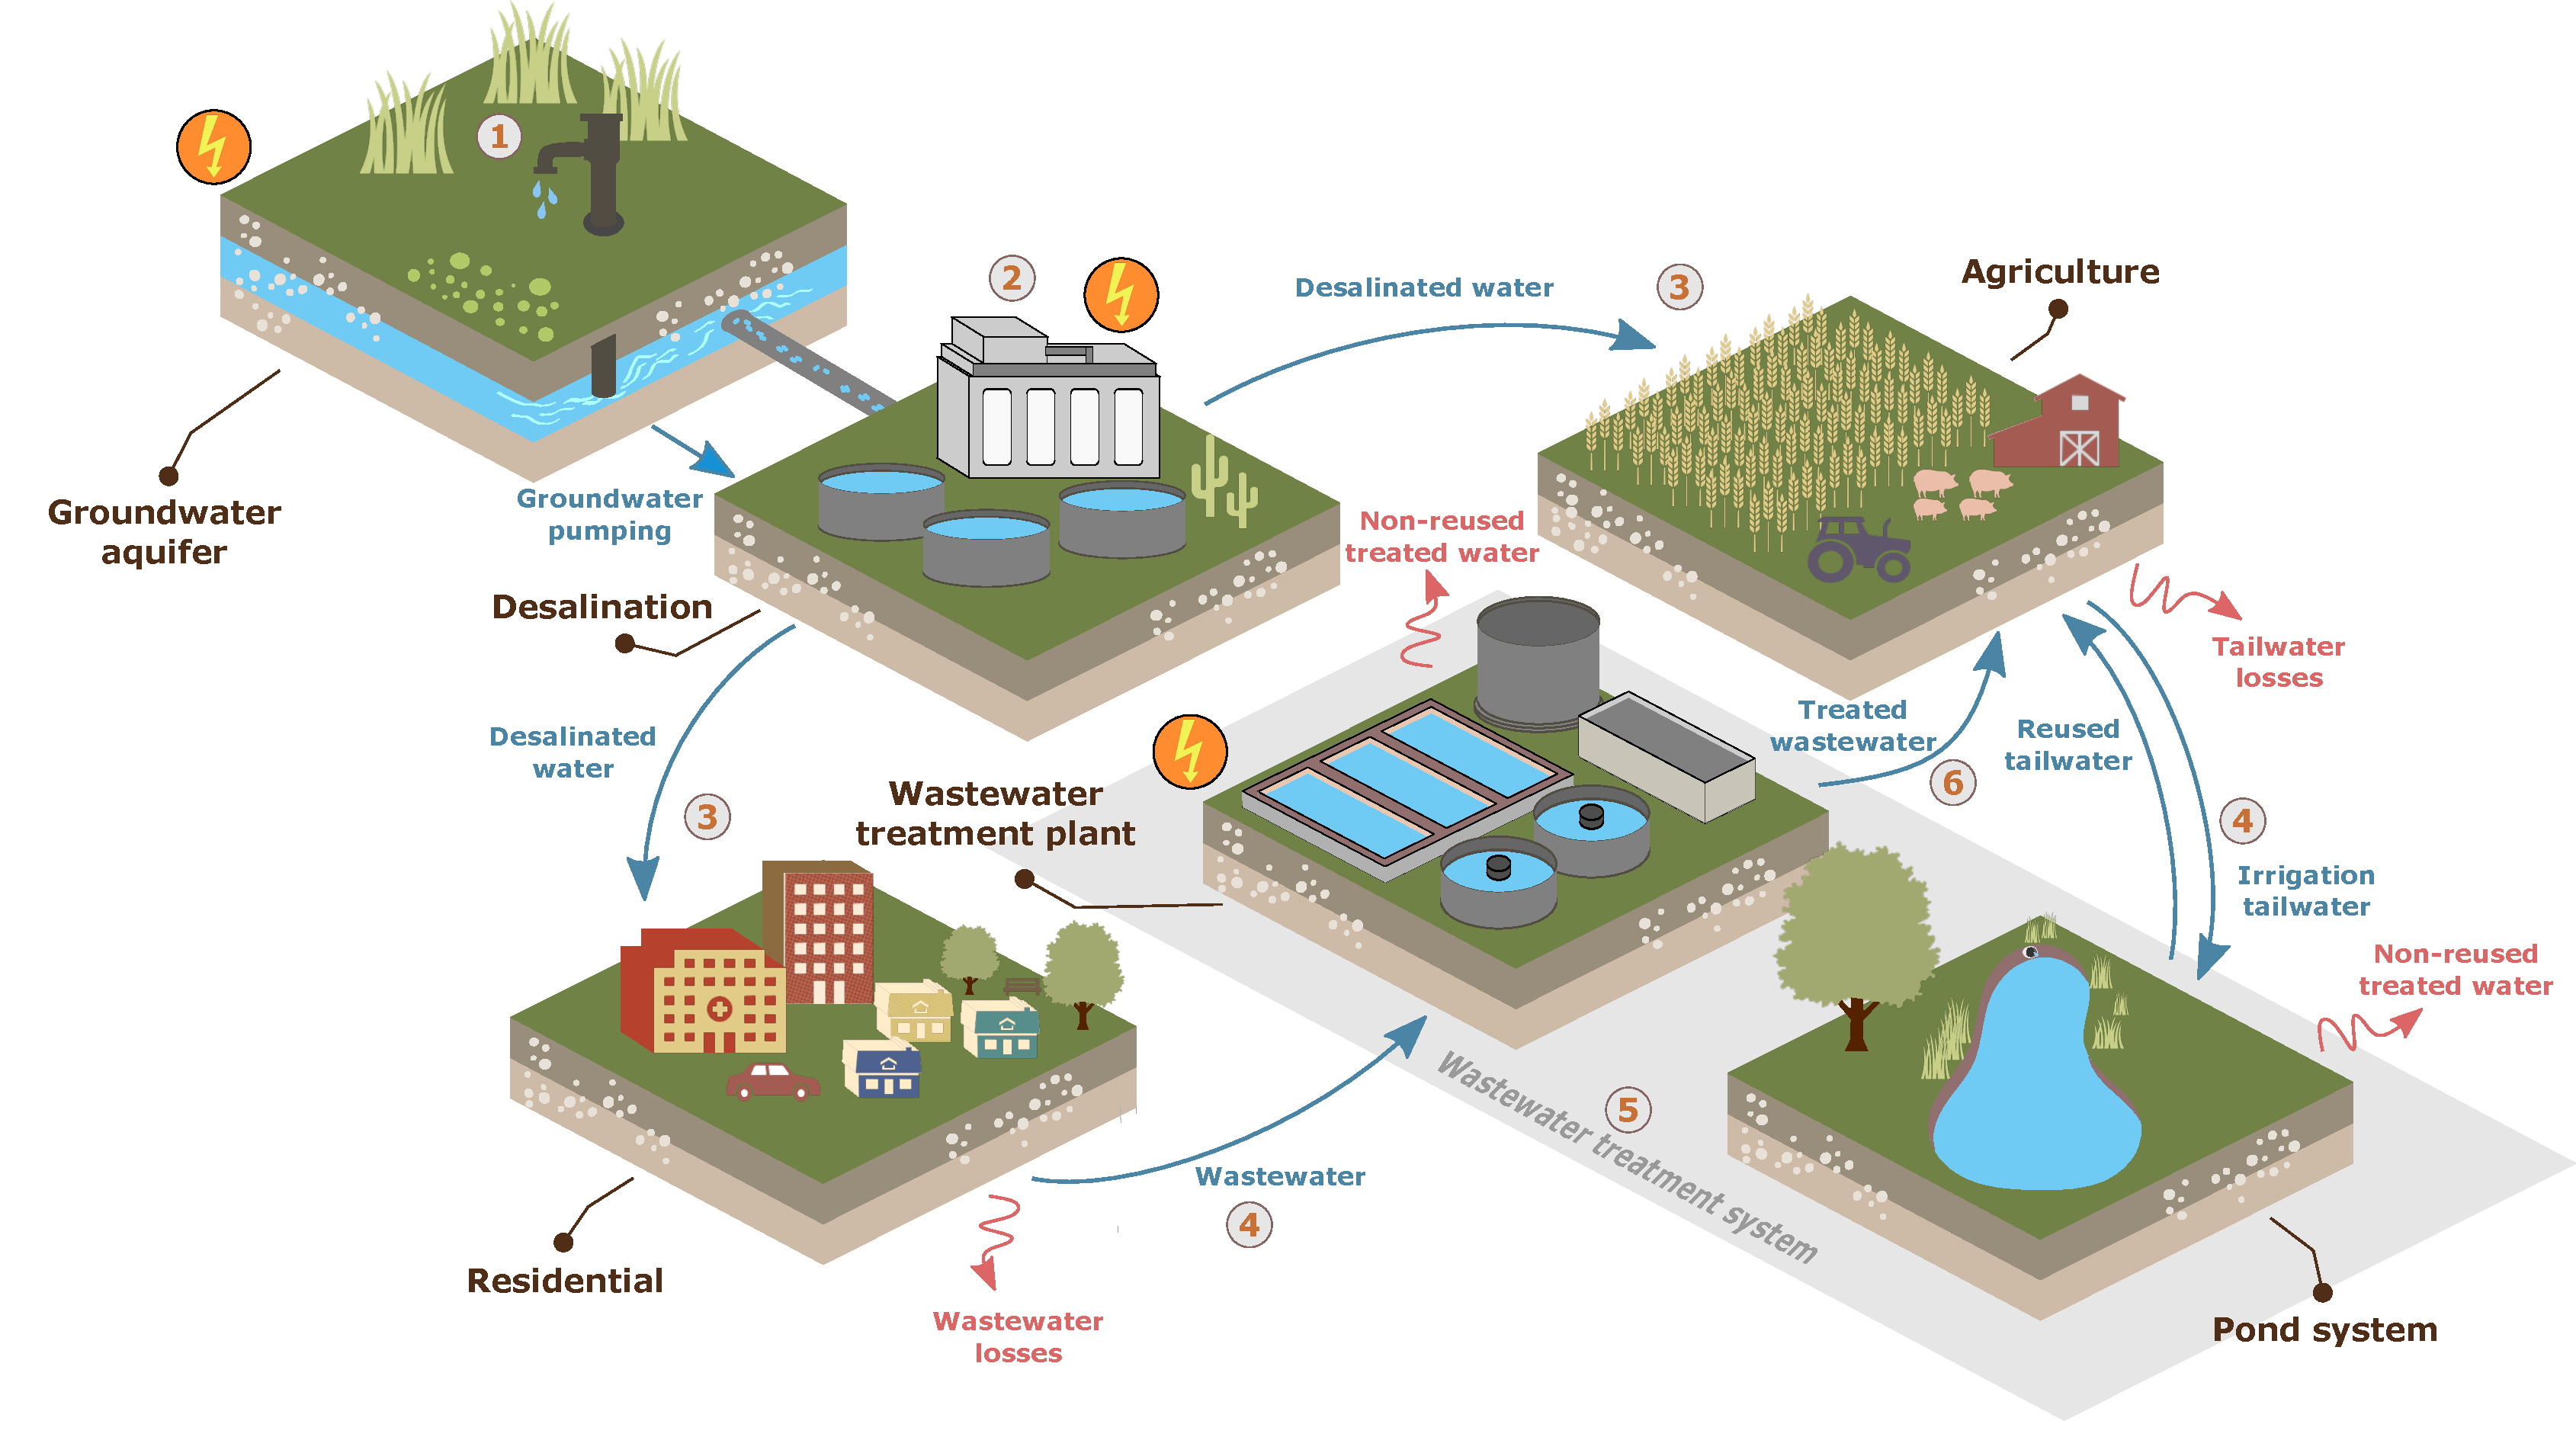
\includegraphics[width=\textwidth]{System_reuse}
	\caption{NWSAS systems, energy and water resource flows. The blocks represent the different systems, the arrows the water flows, the voltage icons the systems that require energy, and the numbers the order of processes.}
	\label{fig:systemreuse}
\end{figure*}
Four wastewater/tailwater treatment and reuse scenarios were analyzed, evaluating current irrigation water pricing regimes and wastewater/tailwater reuse. Irrigation water pricing regimes were taken from \cite{Socioeconomicaspectsirrigation2014}, were it was found that the irrigation water demand per hectare throughout the NWSAS basin is heavily dependent on the supply water cost. Moreover, the same population water demand of 55 m\textsuperscript{3} per capita was used for all scenarios:

\begin{description}
\item[Scenario 1:] This scenario assumes the same behavior as the Baseline, but accounts for wastewater treatment and reuse in irrigation.
\item[Scenario 2:] Private farmers that pay the full price of water without any subsidy. The average level of water demand is around 10,512 m\textsuperscript{3}/ha \cite{Socioeconomicaspectsirrigation2014}. The \citet{Socioeconomicaspectsirrigation2014} found that farmers belonging to this regime have higher water productivity.
\item[Scenario 3:] Users that have access to water subsidized to some extent (``collective" networks). The average water demand is 15,334 m\textsuperscript{3}/ha \cite{Socioeconomicaspectsirrigation2014}.
\item[Scenario 4:] Farmers that have free access to water, meaning that the government fully subsidize the price of water and that the resource can be utilized without limitations. The average irrigation water demand is 21,215 m\textsuperscript{3}/ha \cite{Socioeconomicaspectsirrigation2014}.
\end{description}

\begin{table*}[!b]
    \caption{\label{tbl:methodsScenarios}Brief description and enumeration of additional methods used for the wastewater treatment and reuse scenarios (in order of execution).}
	\footnotesize{
	\begin{tabular}{@{}l P{1.1in} P{1.2in} P{3.12in}}
		\br
		\# & Method & Systems involved & Description\\
	    \mr
	    7. & Desalination energy & Desalination system & Minimum energy requirements to desalinate brackish water using the Reverse Osmosis (RO) process. The TDS content of the water and the water withdrawals of each location are used, plus a minimum TDS content threshold of 1000 mg/l to desalinate (a sensitivity analysis on these parameters were performed) \\
	    8. & Reclaimed, treated and reused wastewater & Residential, agriculture and wastewater treatment system & Estimates the available wastewater and tailwater to be reclaimed. Losses are subtracted and available treated wastewater/tailwater are computed for each cluster \\
	    \ms
	    9. & CAPEX and OPEX estimation & Residential, agriculture and wastewater treatment system & The Capital Expenditure (CAPEX) and the Operational Expenses (OPEX) of each evaluated wastewater treatment system are calculated for each cluster \\
	    \ms
	    10. & LCOW estimation & Wastewater treatment system & The levelized Cost of Water (LCOW) is calculated for each wastewater treatment system in each cluster\\
	    \ms
	    11. & Least-cost option & Wastewater treatment system & The least-cost wastewater treatment options are identified in each cluster\\
	    \ms
	    12. & Recalculate water withdrawals & Groundwater aquifer, residential, agriculture and wastewater treatment system & Based on water demand  from the residential and agricultural sectors and the available treated wastewater for reuse in agriculture in each cluster\\
	    \ms
	    13. & Recalculate groundwater stress & Groundwater aquifer & New groundwater stress indicator based on new water withdrawals after treated wastewater/tailwater reuse in agriculture \\
	    \ms
	    14. & Recalculate pumping and desalination energy & Groundwater aquifer and desalination system & Recalculate pumping and desalination energy requirements for new water withdrawals from the aquifer after treated wastewater reuse in agriculture\\
	    \ms
	    15. & Wastewater treatment energy & Wastewater treatment system & Calculate the energy requirements for wastewater treatment of the least-cost treatment systems selected in each cluster\\
		\br
	\end{tabular}
	}
\end{table*}

It is worth noting that the large irrigation water demand increase seen in the subsidized and free regimes compared to the private regime, suggests a strong price elasticity of the irrigation water demand and/or the use of lower efficiency irrigation technologies in such regimes \cite{Socioeconomicaspectsirrigation2014}.

Although the majority of farmers in the NWSAS are currently under the private water regime, the three water regimes were used as central point of the scenarios with the aim of exploring extremes and highlight the WEF Nexus implications that certain water use behaviors may pose. 

The treated wastewater reuse system analyzed consisted of: 1) extracting water from groundwater resources, 2) desalinating brackish water when needed, 3) supplying water demand for domestic and agricultural irrigation purposes, 4) reclaiming domestic wastewater and agricultural drainage (i.e. tailwater), 5) treating reclaimed wastewater, and 6) reusing treated wastewater in agricultural irrigation. A schematic of the system is presented in \fref{fig:systemreuse}. The same period of 35 years spanning from year 2015 to 2050 was used and results reported for an average year.

% \begin{table*}[!ht]
%     \caption{\label{tbl:scenarios}Description of scenarios based on agricultural water use behaviour. Based on information from \cite{Socioeconomicaspectsirrigation2014}.}
% 	\footnotesize{
% 	\begin{tabular*}{\textwidth}{@{}l P{5.3in}}
% 		\br
% 		Scenario & Description\\
% 		\mr
% 		Scenario 1 & This scenario assumes the same behavior as the Baseline, but implements the wastewater treatment and reuse in irrigation measure.\\
% 		Scenario 2 & Private farmers that pay the full price of water without any subsidy. The average level of water demand is around 10,512 m\textsuperscript{3}/ha \cite{Socioeconomicaspectsirrigation2014}. The \citet{Socioeconomicaspectsirrigation2014} found, that farmers belonging to this regime, have higher water productivity. Moreover, the same population water demand of 55 m\textsuperscript{3} per capita was used and the wastewater treatment and reuse in irrigation measure.\\ 
% 		Scenario 3 & Users that have access to water subsidized to some extent (``collective" networks). The average water demand is 15,334 m\textsuperscript{3}/ha \cite{Socioeconomicaspectsirrigation2014}. Moreover, the same population water demand of 55 m\textsuperscript{3} per capita was used and the wastewater treatment and reuse in irrigation measure.\\
% 		Scenario 4 & Farmers that have free access to water, meaning that the government fully subsidize the price of water and that the resource can be utilized without limitations. The average irrigation water demand is 21,215 m\textsuperscript{3}/ha \cite{Socioeconomicaspectsirrigation2014}. Moreover, the same population water demand of 55 m\textsuperscript{3} per capita was used and the wastewater treatment and reuse in irrigation measure.\\
% % 		High population water & An average water consumption per capita of 73 m\textsuperscript{3}/year \cite{Householdwaterconsumption2014}.\\
% % 		Low population water & An average water consumption per capita of 55 m\textsuperscript{3}/year \cite{Householdwaterconsumption2014}.\\
% 		\br
% 	\end{tabular*}
% 	}
% \end{table*}

The same six steps used to characterize the Baseline were used for the treated wastewater reuse scenarios (see \tref{tbl:methodsBaseline}), plus 9 additional steps which assessed the WEF impact of reusing treated wastewater on the basin (\tref{tbl:methodsScenarios}).

% Brackish water desalination was set to be needed whenever the TDS levels were above 1,000 mg/l, which ensures low impact levels on cropland production \cite{fao1985water} (More details on \textit{section 7} of the \textit{supplementary information}). A further sensitivity analysis on the TDS content threshold to desalinate was performed (see \autoref{sec:sensitivity}). 

\subsection{Clustering algorithm}\label{Sc:clustering}
A clustering approach was used in order to identify dense areas where a wastewater treatment system could be implemented, minimizing constraints imposed by existent large distances among scatter population or irrigated lands. A hierarchical clustering  algorithm was run using the \textit{Agglomerative Clustering} object from the Python \textit{scikit-learn} package \cite{scikit-learn}.

% \begin{figure*}[!b]
%     \centering
% 	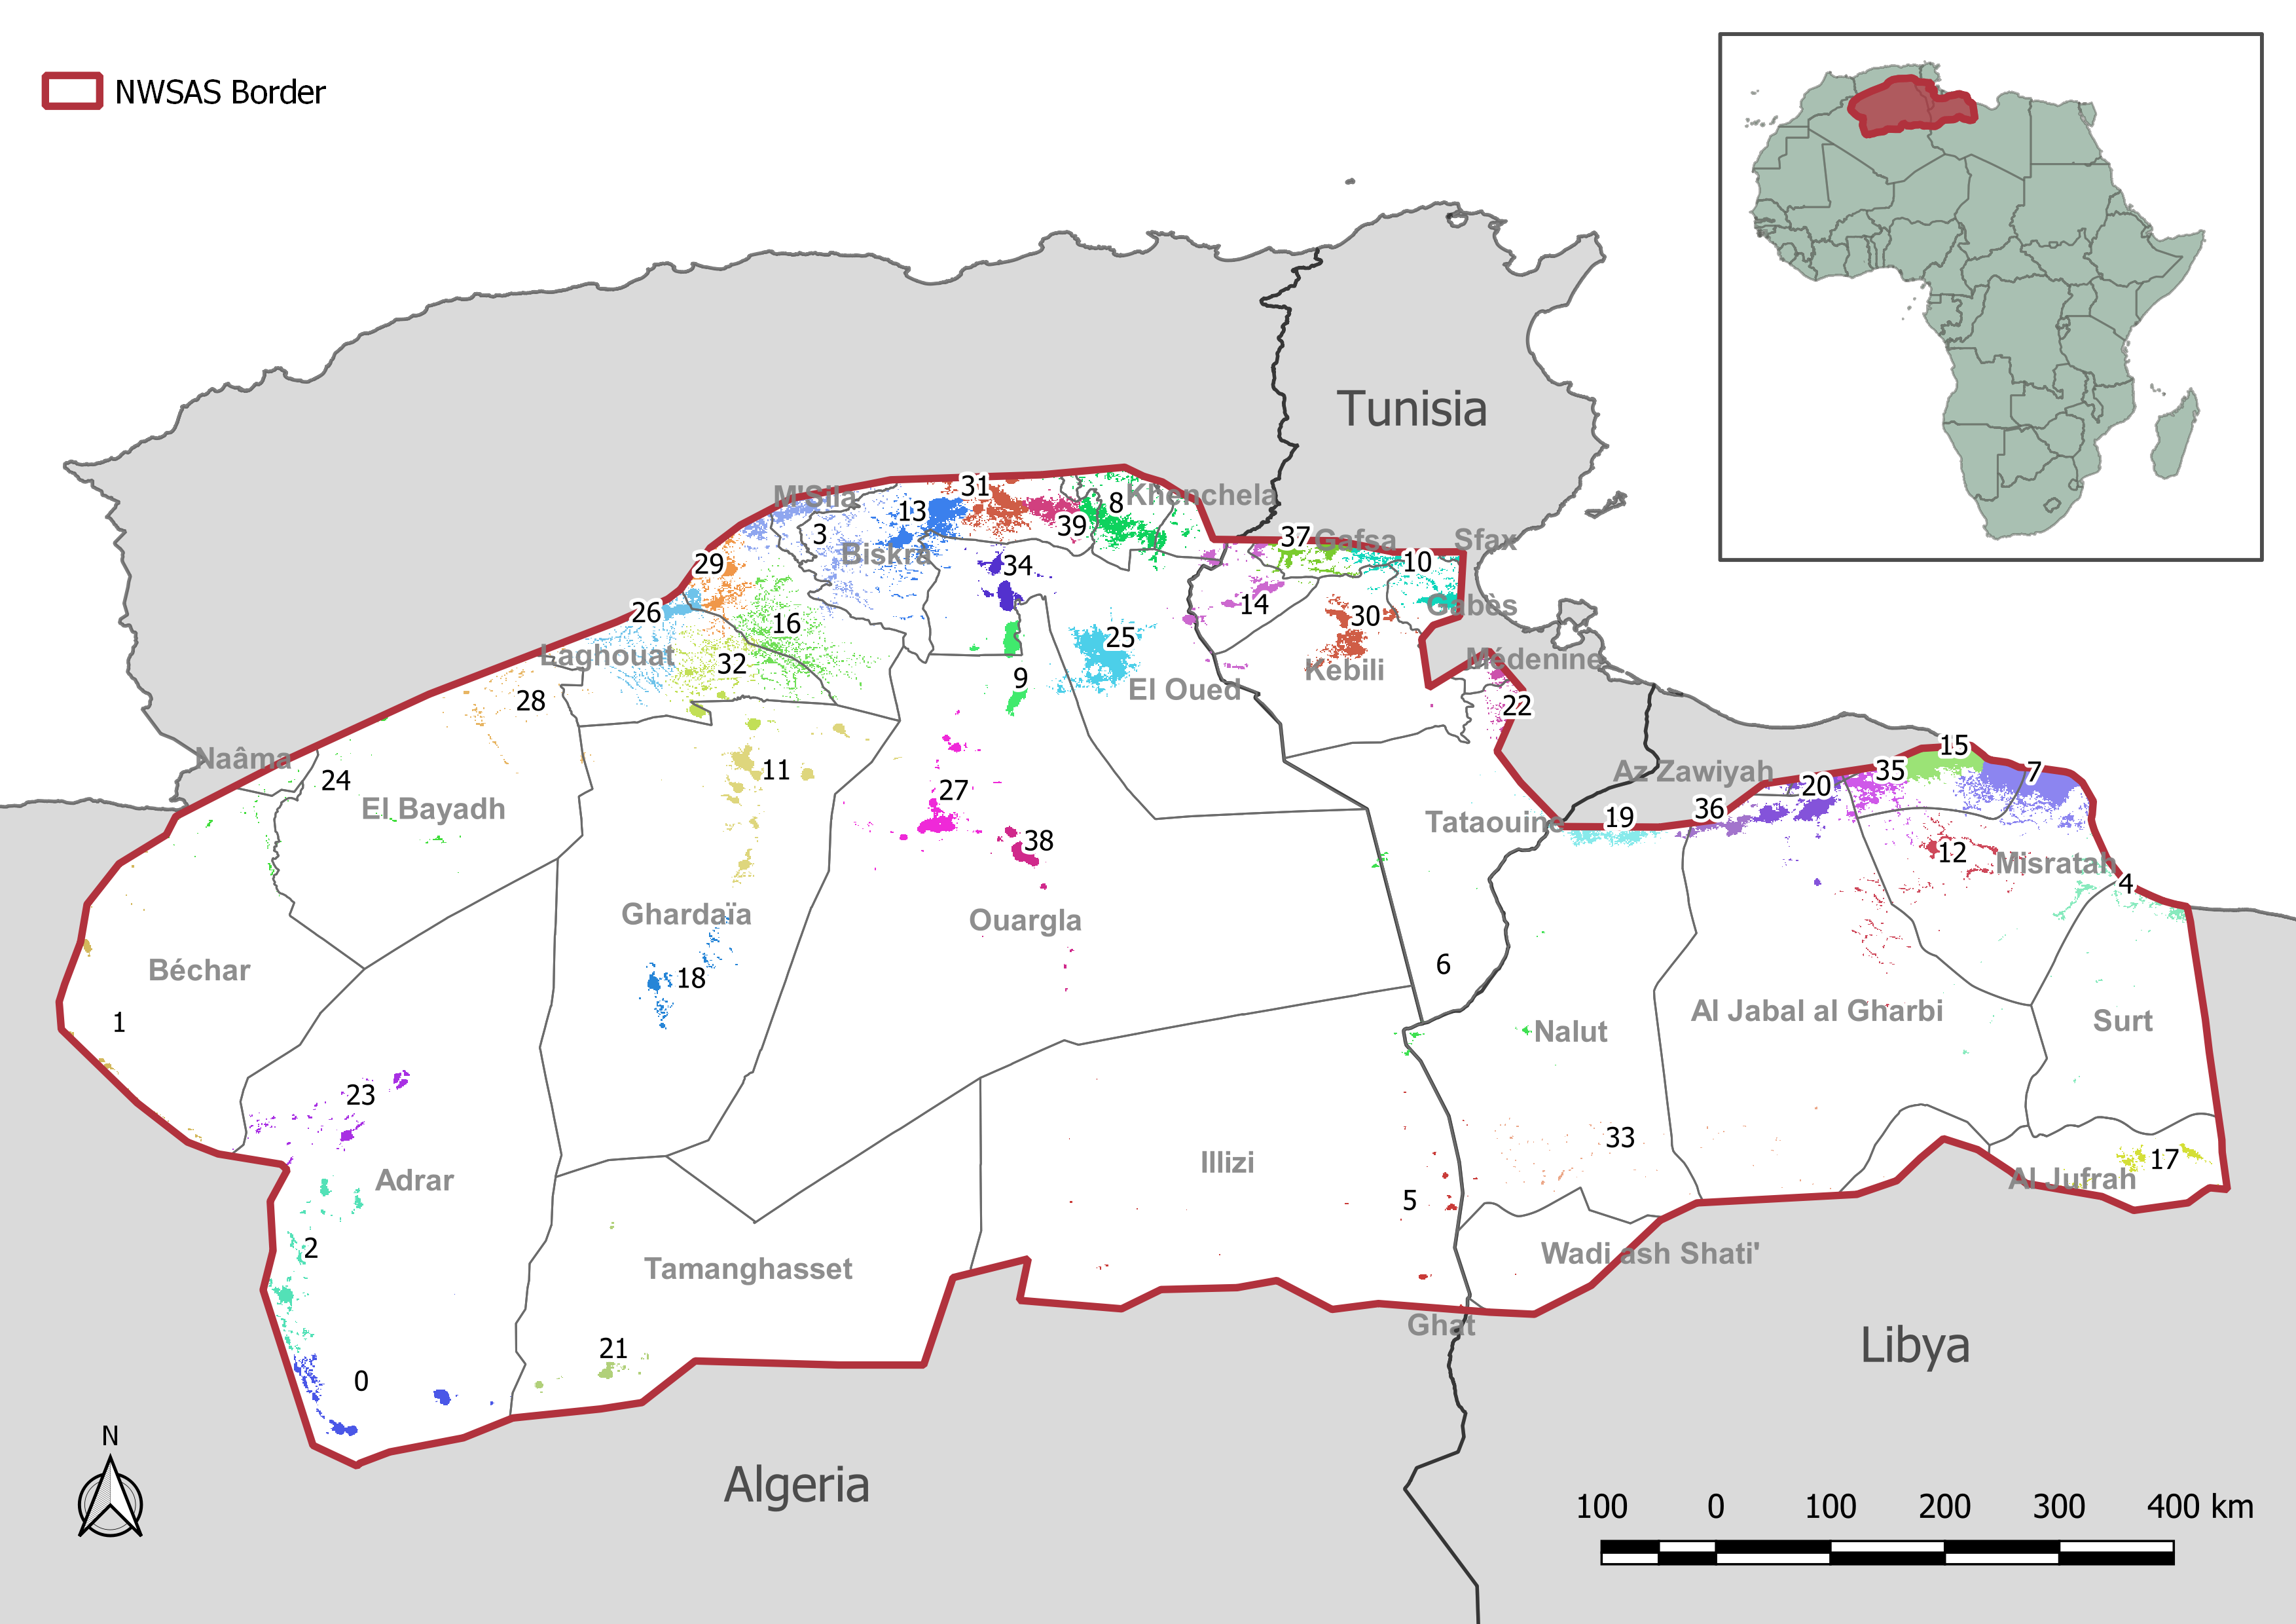
\includegraphics[width=0.88\textwidth, cfbox=black 1pt 0pt]{NWSAS_clusters}
% 	\caption{Population and cropland clusters. Clusters are numbered from 0 to 39, yielding 40 agglomerations including each population and cropland areas. Every cluster is tagged with a number and colored to make them stand out from others. The grey administrative boundaries correspond to the different provinces.}
% 	\label{fig:clusters}
% \end{figure*}

Forty clusters were created in the process, which succeeded in identifying dense agglomerations. When compared with a traditional approach of performing an analysis on a province basis, the clusters achieved a reduction of 360\% on the overall distance between points. This is especially important in larger provinces with substantial population and agricultural activity as Adrar, Ghardaïa, Ouargla and el Oued. Detailed maps of the identified clusters are available in the \textit{supplementary information}.
% Moreover, with this approach, the administrative border constraint is eliminated, as can be seen with cluster number 9 where the agglomeration shares areas from the Ouargla and El Oued provinces.

\subsection{Groundwater Stress Indicator}
The Groundwater Stress Indicator (GWS) was used to quantify the current stress of the aquifer \cite{gleesonWaterBalanceGlobal2012,Aqueductglobalmaps2015}. It relates the ratio of water withdrawals due to anthropogenic reasons (i.e. in this case domestic and irrigation uses), and the total recharge rate of the aquifer. The groundwater stress indicator is usually calculated as the ratio of groundwater footprint to aquifer area \cite{gleesonWaterBalanceGlobal2012,RegionalGroundwaterStress2013}:

\begin{equation}\label{eq:gws} 
GWS = \frac{GF}{A_{A}}
\end{equation}
Where:
\begin{itemize}[label={-}, topsep=2pt,noitemsep]
	\item $GWS$: Groundwater Stress indicator. Values below 1 indicate low stress areas, values from 1 to 5 indicate low to middle stressed areas, values from 5 to 10 indicate middle to high stressed areas, values from 10 to 20 indicate high stressed areas and values above 20 indicate extremely high stressed areas.
	\item $GF$: groundwater footprint. Identifies the right balance between groundwater use and groundwater replenishment for an area.
	\item $A_A$: areal extent of an aquifer throughout a given region.
\end{itemize}~

The groundwater footprint is calculated as:
\begin{equation}\label{eq:gf} 
GF = \frac{C}{R-E}\cdot A
\end{equation}
Where:
\begin{itemize}[label={-}, topsep=2pt,noitemsep]
	\item $C$: total area-averaged annual withdrawals of groundwater for anthropogenic use.
	\item $R$: total area-averaged annual recharge rate of water for groundwater aquifer, including natural and anthropogenic sources.
	\item $E$: total area-averaged annual environmental stream flow used to sustain ecosystem services (assumed as zero for the NWSAS).
	\item $A$: areal extent of a given region where $C$, $R$, and $E$ can be defined.
\end{itemize}

\subsection{Irrigation tailwater treatment system}
Irrigation tailwater capturing, storing and reusing potential were estimated according to \Eref{eq:storage}. 

\begin{equation}\label{eq:storage} 
water_{stored} = 0.8\ water_{used} - water_{crop} - water_{loses}
\end{equation}
Where:
\begin{itemize}[label={-}, topsep=2pt,noitemsep]
	\item $water_{stored}$: monthly water used for irrigation based on each scenario water use regime.
	\item $water_{crop}$: monthly water requirements of the croplands, calculated based on the Penman-Monteith method.
	\item $water_{loses}$ monthly water losses due to evaporation in the storage system, leakage and storage capacity.
\end{itemize}

Crop water requirements ($water_{crop}$) were estimated using the FAO-56 Penman-Monteith method for evapotranspiration \cite{allenFAOIrrigationDrainage1998}. Meteorological parameters were calculated from ``WorldClim" monthly data \cite{WorldClimGlobalClimate}  using the Python library ``Pyeto" \cite{pyeto}. For the purpose of this study, date palms and vegetables were assumed to cover in equal shares the cropland area---as they represent the main crops cultivated in the region \cite{almullaNWSAS,Socioeconomicaspectsirrigation2014}. The crop coefficients and irrigation calendar were set according to \cite{almullaNWSAS}. From this process, the monthly crop water needs throughout the entire basin were obtained.

Furthermore, an on-farm storage pond system was evaluated to account for the potential reusable water ($water_{stored}$). For this, a water balance on the on-farm storage was executed following a similar approach to \citet{reinhartSimulatedWaterQuality2019}. First, the maximum attainable irrigation efficiency (i.e. crop water requirements over irrigation water used) was set to be 80\%, being the remaining 20\% non-recoverable loses. If additional water was available, it was recovered and stored. The storage reservoir surface area, was assumed at 2\% of the cropland area and a standard depth of 3 meters \cite{reinhartSimulatedWaterQuality2019}. Leakage losses in the storage system were set to be 0.9 mm/day, and evaporation loses were calculated using a modified Penman-Monteith method for an open water body \cite{reinhartSimulatedWaterQuality2019}. For this, and albedo, surface height, and surface roughness values of 0.05, 0.002 m, and 0 s/m, respectively were used \cite{princeczarneckijobym.QuantifyingCaptureUse2017}. Moreover, energy requirements of 0.19 kWh/m\textsuperscript{3} of tailwater conveyed was used.

\subsection{Domestic wastewater treatment system}
The amount of domestic wastewater generated, was assumed to represent around 70\% of the total domestic water used \cite{unescoWastewaterUntappedResource2017}. From that share, an additional 10\% was assumed to be lost in the capture, conveyance and treatment processes. Pollutant levels of domestic wastewater were assumed to be constant throughout the basin, using standard values based on studies from FAO \cite{fao1985water}. Such levels and the required levels for reused treated wastewater in irrigation are shown in \tref{tbl:pollutans}.
% \textit{section 6} of the \textit{supplementary information}.

\begin{table*}[!ht]
	\caption{\label{tbl:pollutans}Pollutant levels of domestic wastewater and treated wastewater to be reused in agricultural irrigation. Based on \cite{fao1985water}.}
    \footnotesize
	\begin{tabular}{@{}*{4}l}
	\br
		Pollutant type & Domestic (mg/l) & Treated (mg/l) & Removal (\%)\\
		\mr
		Suspended solids ($SS$) & 700 & 30 & 95\\
		Nitrogen ($N$) & 40 & 30 & 25\\
		Phosphorus ($P$) & 20 & 10 & 50\\
		Biochemical Oxygen Demand ($BOD_5$) & 500 & 50 & 90\\
		Chemical Oxygen Demand ($COD$)& 1300 & 120 & 90\\
		\br
	\end{tabular}
\end{table*}

One irrigation tailwater treatment technology and seven domestic secondary Wastewater Treatment Technologies (WWTT) were evaluated (\tref{tbl:treatmentsystems}). For this, pollutant removal ranges, capital and operational costs were taken into account. Cost functions in terms of wastewater treatment capacity, were used for each technology to estimate Capital Expenditure (CAPEX) (i.e. includes all capital investments required) and Operational Expenses (OPEX) (i.e. covers all fix and variable costs needed to operate the plant, including energy requirements) \cite{Costmodellingwastewater2011,Assessmentwastewatertreatment2012,Economicfeasibility2012}. However, technology specific cost functions were not available for the NWSAS basin area, nor statistical data to develop them. Therefore, based on the work of \citet{Assessmentwastewatertreatment2012} cost functions for different WWTTs in Spain were used to evaluate the competence of selected technologies in the NWSAS. Moreover, energy intensity characteristics were added for each technology according to \cite{Energypatternanalysis2012,ComparativeAnalysisEnergy2017}. See \textit{section 6} of the \textit{supplementary information} for specific information of the evaluated technologies.

\begin{table*}[!ht]
	\caption{\label{tbl:treatmentsystems}Domestic wastewater treatment systems analysed.}
    \begin{indented}
	\item[]\begin{tabular}{@{}*{3}l}
	\br
		Technology & Usage & Energy (kWh/m\textsuperscript{3})\\
		\mr
		Intermittent Sand Filter (ISF) & Domestic wastewater & 0.2\\
		Trickling Filter (TF) & Domestic wastewater & 0.3\\
		Moving Bed Biofilm Reactor (MBBR) & Domestic wastewater & 0.8\\
		Rotating Biological Contractors (RBC) & Domestic wastewater & 0.8\\
		Membrane Bioreactor (MBR) & Domestic wastewater & 0.8\\
		Extended Aeration (EA) & Domestic wastewater & 0.6\\
		Sequencing Batch Reactor (SBR) & Domestic wastewater & 1.0\\
		\br
	\end{tabular}
	\end{indented}
\end{table*}

\subsection{Levelized Cost of Water}
A proposed LCOW method was used as a metric to compare cost-effectiveness among WWTTs. The LCOW assesses the life-cycle cost of delivering one unit (e.g. one cubic meter) of treated wastewater, based on all physical assets and resources required \cite{ISI:000209031000003}. This concept, is inherited from the Levelized Cost of Electricity (LCOE) methodology, which applies the same life-cost analysis for one unit of electricity output \cite{prospectscostcompetitive2013}. The LCOW method follows the logic of the LCOE method \cite{prospectscostcompetitive2013,GeospatialLevelizedCost2015}, with pertinent adjustments to the variables used in wastewater treatment systems. The project life span was set for 35 years, covering the period from 2015 to 2050. Then, the LCOW can be expressed as follows:

\begin{equation}\label{eq:lcow}
LCOW = LCOW_{Inv} + LCOW_{O\&M} %+ LCOW_{Ext}
\end{equation}

The expression presented in \eref{eq:lcow}, disaggregates the $LCOW$ (\$/m\textsuperscript{3}) value in two components: the cost components due to investment $LCOW_{Inv}$, and operation and maintenance $LCOW_{O\&M}$. As the CAPEX function comprises all investment components of a wastewater treatment plant, it enables an easy calculation of the $LCOW_{Inv}$ for each WWTT and each region or cluster. \Eref{eq:lcowinv} describes the process to calculate the $LCOW_{Inv}$.

\begin{equation}\label{eq:lcowinv}
LCOW_{Inv} = \frac{Inv}{\sum_{t=1}^{T} V_{t}\cdot\gamma^{t}}\cdot\Delta
\end{equation}

Where $Inv$ stands for the CAPEX value, $V_{t}$ for the treated water flow per year $t$ (m\textsuperscript{3}/yr), $\Delta$ for the tax factor (assumed as 1) and $\gamma^{t}$ represents the discount factor of the project, calculated for a discount rate of 5\%.

The LCOW related to operational costs $LCOW_{O\&m}$ \eref{eq:lcowom} was computed by using the OPEX values $\omega_{t}$ calculated for each year in each cluster and the discount factor $\gamma^t$ per year.

\begin{equation}\label{eq:lcowom}
LCOW_{O\&m} = \frac{\sum_{t=1}^{T} \omega_{t}\cdot\gamma^{t}}{\sum_{t=1}^{T} V_{t}\cdot\gamma^{t}}
\end{equation}

% Furthermore, the avoidance of externalities due to discharge of untreated wastewater into ecosystems, can be accounted by estimating the effects that pollutants presented in wastewater and tailwater stream flows can have into fresh water bodies, rivers or groundwater aquifers (see section 8 of the \textit{supplementary information} for more detail) \cite{Assessmentwastewatertreatment2012}. However, due to lack of information of environmental effects of wastewater pollutants in the region, this parameter was not considered.

\subsection{Sensitivity analysis}\label{sec:sensitivity}
% TODO: write something about the uncertainty of the data being the driver for the sensitivity analysis. That apart from the scenario exploration, we provide sensitivity analysis to capture changes on the input data.
Sensitivity analysis were performed on the following key model parameters in order to provide clarity of the contributions of the inputs to the uncertainty in the results: domestic water use per capita, depth to groundwater levels change, groundwater quality change, irrigated area increase, TDS threshold to desalinate brackish water extracted from the aquifer and discount rate. The complete rationale and results of the sensitivity analysis are reported in section 12 of the \textit{supplementary information}. %TODO: change section name
% domestic per capita water consumption, groundwater quality change, depth to groundwater levels change, irrigated area change, TDS threshold to desalinate brackish water extracted from the aquifer and discount rate (\tref{tbl:sensitivy}). 
% These parameters were selected, as the water security of the aquifer highly depends on them, directly affecting food security.